%
% Chapitre "Structure d'un rapport technique"
%

\chapter{Conceptualisation}
\label{s:conceptualisation}
\section{Diagramme Fonctionnel}
Pour s'assurer de bien répondre aux demandes du client, nous devons tenir compte des intrants et extrants du système conceptualisé. Nous devons aussi penser à des fonctions qui permettront de faire le lien entre ce qui entre dans notre système et ce qui en ressortira. La figure \ref{diagramme_fonctionnel} est une représentation graphique des liens entre les intrants et extrants ainsi que les fonctions intermédiaires entre ceux-ci.

\begin{figure}[p]
    \centering
    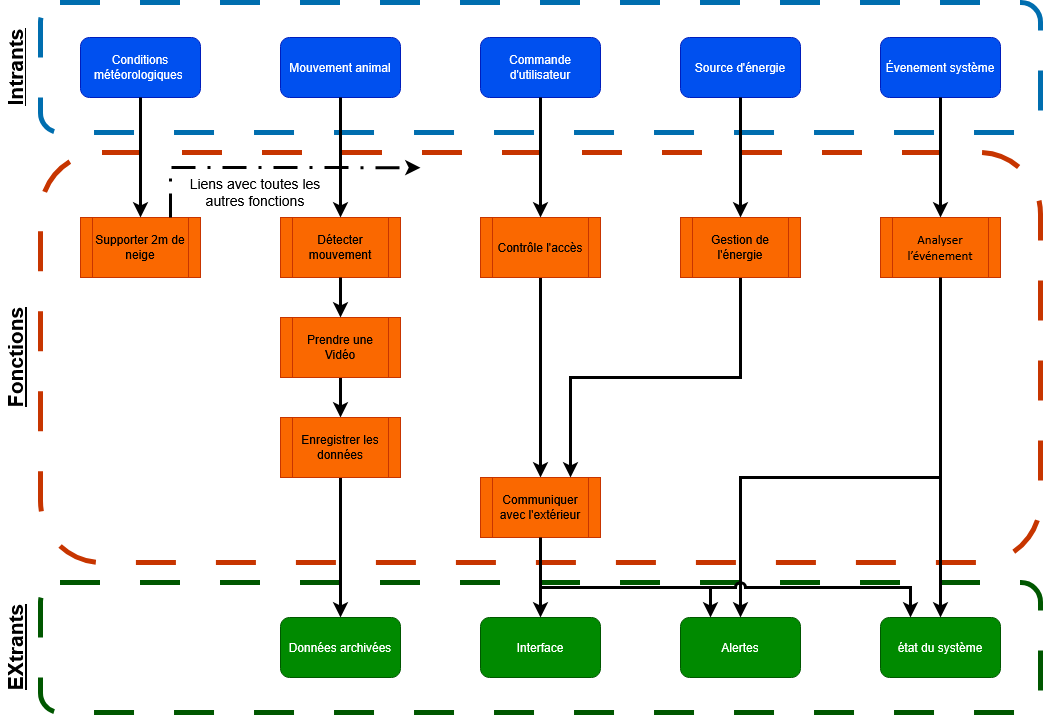
\includegraphics[width=1\textwidth]{fig/diagramme_fonctionnel.png}
    \caption{Diagramme fonctionnel du projet NordFaune}
    \label{diagramme_fonctionnel}
\end{figure}

\section{Conceptualisation des solutions}
\subsection{Prendre une vidéo}
La prise de vidéo est un concept capital du projet NordFaune, puisque les vidéos captées seront utilisées à des fins statiques par la suite. Il est donc important d'assurer une qualité constante de chaque vidéo, en s'assurant toutefois de ne pas dépasser les limites imposées par le système. (Voir \ref{} sur le stockage des données)
\bigskip

\textbf{Aspect physique:}
\begin{itemize}
    \item Le capteur vidéo doit être assez petit pour pouvoir être intégré au système.
    \item Les vidéos captées par l'appareil doivent disposer d'une résolution satisfaisante pour une analyse future.
    \item Doit pouvoir communiquer et interagir avec un ordinateur moderne.
\end{itemize}

\textbf{Aspect économique:}
\begin{itemize}
    \item Le capteur doit être peut couteux.
\end{itemize}

\textbf{Aspect temporel:} N/A

\textbf{Aspect socio-environnemental:}
\begin{itemize}
    \item Ne doit pas interférer avec la faune artique.
\end{itemize}

\subsubsection{GoPro Hero}
\textbf{Description} La caméra Hero de la marque GoPro est une petite caméra très compacte et légère. (56,6 mm de large et 29,4 mm de hauteur) Elle peut enregistrer des vidéos jusqu'à une résolution de 4k à 30 FPS et dispose d'un port microSD pour pouvoir enregistrer les vidéos capturées. Au besoin, elle peut se connecter VIA Wifi, Bluetooth ou tout simplement à l'aide d'un câble USB-C  pour communiquer et transférer ses données vers un ordinateur. La caméra Hero est robuste et étanche jusqu'à une profondeur de 5m. De plus, elle résiste généralement bien au froid, surtout si connectée à une source d'énergie externe. La caméra Hero peut s'acheter facilement sur le site de GoPro ou sur Amazon à un prix d'environ 280\$.

\textbf{Décision} Rejetée

\textbf{Justification} Ce concept a été rejeté, puisque malgré plusieurs caractéristiques intéressantes comme la robustesse et l'étanchéité, le prix de 280\$ est tout simplement trop élevé. De plus, plusieurs caractéristiques de cette caméra sont tout simplement inutiles pour la mise en œuvre du design conceptuel. C'est le cas de la captation vidéo jusqu'à une résolution de 4k qui demande beaucoup d'espace de stockage et qui n'est pas nécessaire pour une bonne analyse des images.

\textbf{Références}
\cite{Gopro1}
\cite{Gopro2}

\subsubsection{ArduCam IMX219}
\textbf{Description} La caméra ArduCam IMX219 est principalement conçue pour permettre une intégration facile avec les ordinateurs Raspberry Pi. Avec son capteur de 8MP, il est possible de prendre des vidéos HD jusqu'à 47 images par seconde. Le module communique directement avec un ordinateur Raspberry Pi par l'intermédiaire de deux lignes MIPI CSI-2. Elle est très compacte et elle sera facile à installer dans la boîte avec les autres composants du système. De plus, puisque c'est seulement un module de caméra dédié uniquement à la prise de photos ou de vidéos, il consomme très peu d'énergie. Avec un prix de 30\$ dur le site de ArduCam ou 40\$ sur Amazon, cette caméra n'est pas dispendieuse et facile à se procurer.

\textbf{Décision} Retenue

\textbf{Justification} Ce concept est retenu, puisqu'il répond aisément à tous les critères. Il n'est pas cher, occupe très peu d'espace et peut enregistrer des vidéos avec une résolution acceptable. Cependant, il est préférable d'utiliser un ordinateur Raspberry avec ce capteur ce qui facilitera son installation et sa mise en marche.

\textbf{Références} 
\cite{Gopro1}
\cite{Gopro2}